% Created by tikzDevice version 0.7.0 on 2014-07-29 02:50:02
% !TEX encoding = UTF-8 Unicode
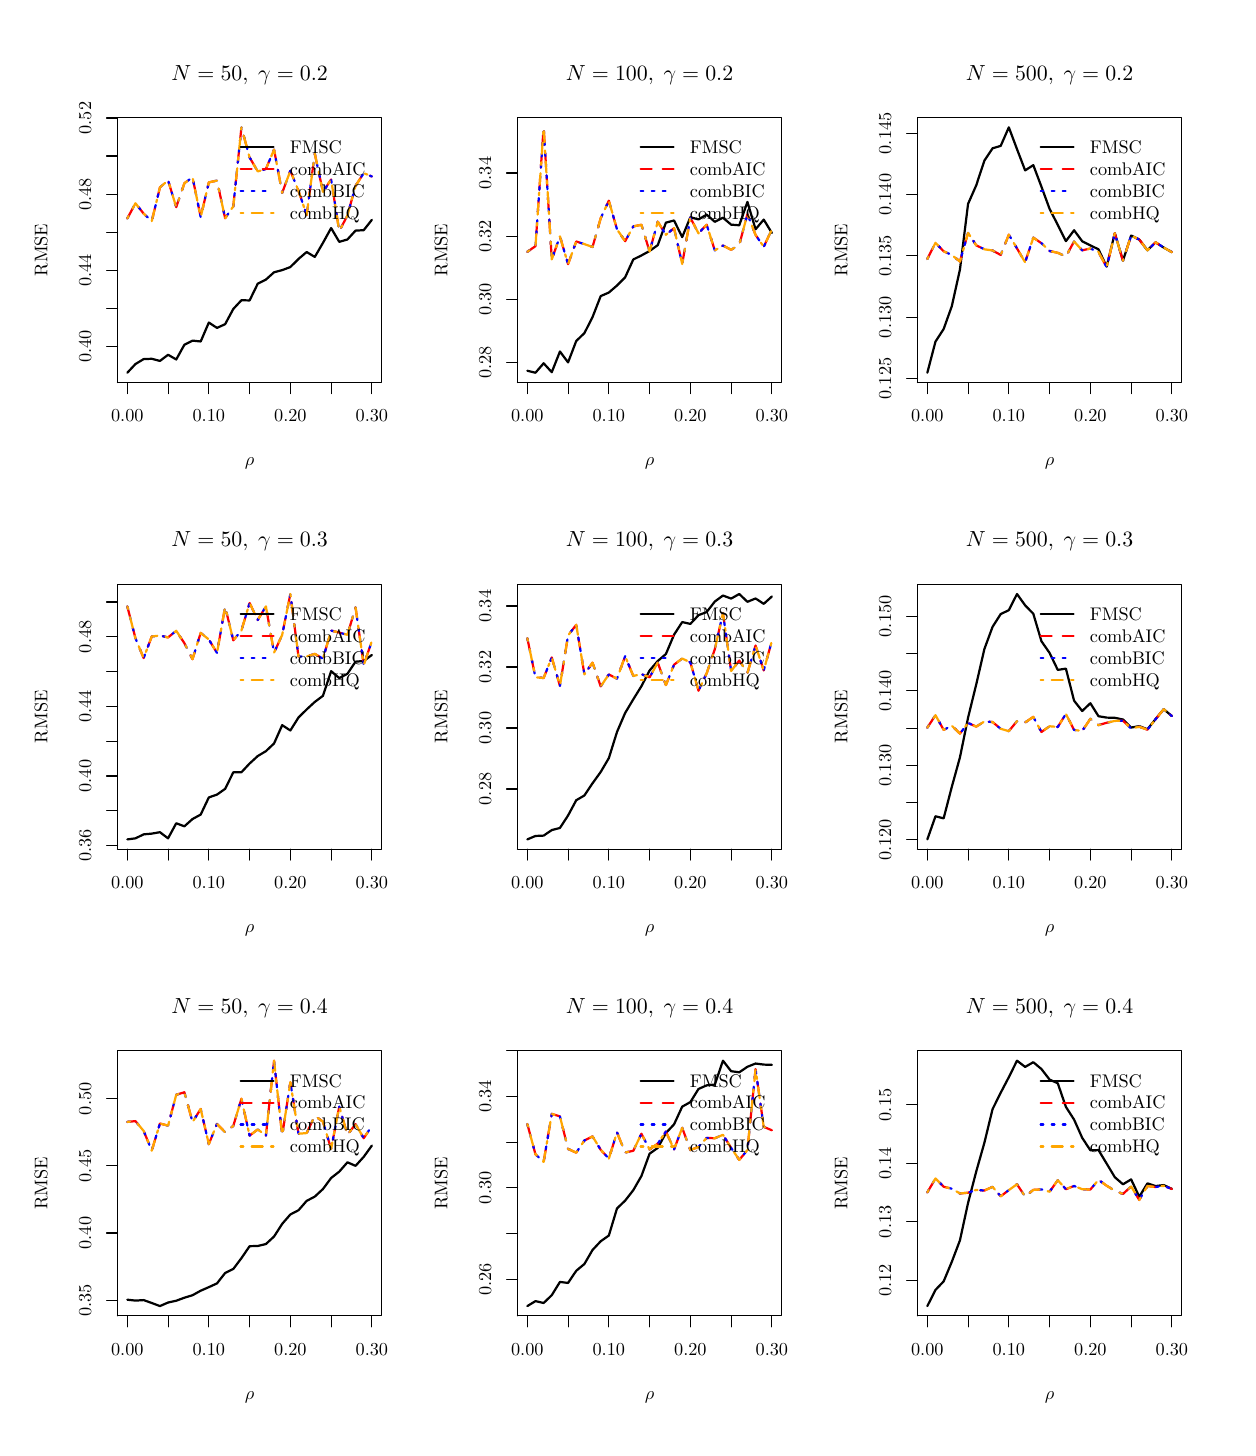
\begin{tikzpicture}[x=1pt,y=1pt]
\definecolor[named]{fillColor}{rgb}{1.00,1.00,1.00}
\path[use as bounding box,fill=fillColor,fill opacity=0.00] (0,0) rectangle (433.62,505.89);
\begin{scope}
\path[clip] ( 32.47,377.65) rectangle (127.91,473.42);
\definecolor[named]{drawColor}{rgb}{0.00,0.00,0.00}

\path[draw=drawColor,line width= 0.8pt,line join=round,line cap=round] ( 36.01,381.20) --
	( 38.95,384.34) --
	( 41.90,386.12) --
	( 44.84,386.24) --
	( 47.79,385.46) --
	( 50.73,387.69) --
	( 53.68,385.99) --
	( 56.63,391.31) --
	( 59.57,392.80) --
	( 62.52,392.49) --
	( 65.46,399.33) --
	( 68.41,397.40) --
	( 71.35,398.74) --
	( 74.30,404.24) --
	( 77.24,407.39) --
	( 80.19,407.32) --
	( 83.14,413.38) --
	( 86.08,414.85) --
	( 89.03,417.50) --
	( 91.97,418.28) --
	( 94.92,419.38) --
	( 97.86,422.31) --
	(100.81,424.82) --
	(103.75,423.04) --
	(106.70,428.12) --
	(109.65,433.47) --
	(112.59,428.49) --
	(115.54,429.35) --
	(118.48,432.55) --
	(121.43,432.71) --
	(124.37,436.45);
\end{scope}
\begin{scope}
\path[clip] (  0.00,  0.00) rectangle (433.62,505.89);
\definecolor[named]{drawColor}{rgb}{0.00,0.00,0.00}

\path[draw=drawColor,line width= 0.4pt,line join=round,line cap=round] ( 36.01,377.65) -- (124.37,377.65);

\path[draw=drawColor,line width= 0.4pt,line join=round,line cap=round] ( 36.01,377.65) -- ( 36.01,373.69);

\path[draw=drawColor,line width= 0.4pt,line join=round,line cap=round] ( 50.73,377.65) -- ( 50.73,373.69);

\path[draw=drawColor,line width= 0.4pt,line join=round,line cap=round] ( 65.46,377.65) -- ( 65.46,373.69);

\path[draw=drawColor,line width= 0.4pt,line join=round,line cap=round] ( 80.19,377.65) -- ( 80.19,373.69);

\path[draw=drawColor,line width= 0.4pt,line join=round,line cap=round] ( 94.92,377.65) -- ( 94.92,373.69);

\path[draw=drawColor,line width= 0.4pt,line join=round,line cap=round] (109.65,377.65) -- (109.65,373.69);

\path[draw=drawColor,line width= 0.4pt,line join=round,line cap=round] (124.37,377.65) -- (124.37,373.69);

\node[text=drawColor,anchor=base,inner sep=0pt, outer sep=0pt, scale=  0.66] at ( 36.01,363.40) {0.00};

\node[text=drawColor,anchor=base,inner sep=0pt, outer sep=0pt, scale=  0.66] at ( 65.46,363.40) {0.10};

\node[text=drawColor,anchor=base,inner sep=0pt, outer sep=0pt, scale=  0.66] at ( 94.92,363.40) {0.20};

\node[text=drawColor,anchor=base,inner sep=0pt, outer sep=0pt, scale=  0.66] at (124.37,363.40) {0.30};

\path[draw=drawColor,line width= 0.4pt,line join=round,line cap=round] ( 32.47,390.68) -- ( 32.47,473.26);

\path[draw=drawColor,line width= 0.4pt,line join=round,line cap=round] ( 32.47,390.68) -- ( 28.51,390.68);

\path[draw=drawColor,line width= 0.4pt,line join=round,line cap=round] ( 32.47,404.44) -- ( 28.51,404.44);

\path[draw=drawColor,line width= 0.4pt,line join=round,line cap=round] ( 32.47,418.21) -- ( 28.51,418.21);

\path[draw=drawColor,line width= 0.4pt,line join=round,line cap=round] ( 32.47,431.97) -- ( 28.51,431.97);

\path[draw=drawColor,line width= 0.4pt,line join=round,line cap=round] ( 32.47,445.74) -- ( 28.51,445.74);

\path[draw=drawColor,line width= 0.4pt,line join=round,line cap=round] ( 32.47,459.50) -- ( 28.51,459.50);

\path[draw=drawColor,line width= 0.4pt,line join=round,line cap=round] ( 32.47,473.26) -- ( 28.51,473.26);

\node[text=drawColor,rotate= 90.00,anchor=base,inner sep=0pt, outer sep=0pt, scale=  0.66] at ( 22.97,390.68) {0.40};

\node[text=drawColor,rotate= 90.00,anchor=base,inner sep=0pt, outer sep=0pt, scale=  0.66] at ( 22.97,418.21) {0.44};

\node[text=drawColor,rotate= 90.00,anchor=base,inner sep=0pt, outer sep=0pt, scale=  0.66] at ( 22.97,445.74) {0.48};

\node[text=drawColor,rotate= 90.00,anchor=base,inner sep=0pt, outer sep=0pt, scale=  0.66] at ( 22.97,473.26) {0.52};

\path[draw=drawColor,line width= 0.4pt,line join=round,line cap=round] ( 32.47,377.65) --
	(127.91,377.65) --
	(127.91,473.42) --
	( 32.47,473.42) --
	( 32.47,377.65);
\end{scope}
\begin{scope}
\path[clip] (  0.00,337.26) rectangle (144.54,505.89);
\definecolor[named]{drawColor}{rgb}{0.00,0.00,0.00}

\node[text=drawColor,anchor=base,inner sep=0pt, outer sep=0pt, scale=  0.79] at ( 80.19,486.92) {\bfseries $N=50, \;\gamma=0.2$};

\node[text=drawColor,anchor=base,inner sep=0pt, outer sep=0pt, scale=  0.66] at ( 80.19,347.56) {$\rho$};

\node[text=drawColor,rotate= 90.00,anchor=base,inner sep=0pt, outer sep=0pt, scale=  0.66] at (  7.13,425.53) {RMSE};
\end{scope}
\begin{scope}
\path[clip] ( 32.47,377.65) rectangle (127.91,473.42);
\definecolor[named]{drawColor}{rgb}{1.00,0.00,0.00}

\path[draw=drawColor,line width= 0.8pt,dash pattern=on 4pt off 4pt ,line join=round,line cap=round] ( 36.01,436.95) --
	( 38.95,442.43) --
	( 41.90,438.70) --
	( 44.84,435.97) --
	( 47.79,448.16) --
	( 50.73,450.73) --
	( 53.68,441.03) --
	( 56.63,449.68) --
	( 59.57,451.83) --
	( 62.52,437.41) --
	( 65.46,449.98) --
	( 68.41,450.63) --
	( 71.35,437.01) --
	( 74.30,441.32) --
	( 77.24,469.87) --
	( 80.19,459.00) --
	( 83.14,453.95) --
	( 86.08,454.83) --
	( 89.03,461.80) --
	( 91.97,446.22) --
	( 94.92,454.18) --
	( 97.86,446.93) --
	(100.81,438.20) --
	(103.75,460.35) --
	(106.70,446.55) --
	(109.65,451.02) --
	(112.59,432.39) --
	(115.54,438.01) --
	(118.48,448.73) --
	(121.43,453.33) --
	(124.37,452.11);
\definecolor[named]{drawColor}{rgb}{0.00,0.00,1.00}

\path[draw=drawColor,line width= 0.8pt,dash pattern=on 1pt off 3pt ,line join=round,line cap=round] ( 36.01,436.95) --
	( 38.95,442.43) --
	( 41.90,438.70) --
	( 44.84,435.97) --
	( 47.79,448.16) --
	( 50.73,450.73) --
	( 53.68,441.03) --
	( 56.63,449.68) --
	( 59.57,451.83) --
	( 62.52,437.41) --
	( 65.46,449.98) --
	( 68.41,450.63) --
	( 71.35,437.01) --
	( 74.30,441.32) --
	( 77.24,469.87) --
	( 80.19,459.00) --
	( 83.14,453.95) --
	( 86.08,454.83) --
	( 89.03,461.80) --
	( 91.97,446.22) --
	( 94.92,454.18) --
	( 97.86,446.93) --
	(100.81,438.20) --
	(103.75,460.35) --
	(106.70,446.55) --
	(109.65,451.02) --
	(112.59,432.39) --
	(115.54,438.01) --
	(118.48,448.73) --
	(121.43,453.33) --
	(124.37,452.11);
\definecolor[named]{drawColor}{rgb}{1.00,0.65,0.00}

\path[draw=drawColor,line width= 0.8pt,dash pattern=on 1pt off 3pt on 4pt off 3pt ,line join=round,line cap=round] ( 36.01,436.95) --
	( 38.95,442.43) --
	( 41.90,438.70) --
	( 44.84,435.97) --
	( 47.79,448.16) --
	( 50.73,450.73) --
	( 53.68,441.03) --
	( 56.63,449.68) --
	( 59.57,451.83) --
	( 62.52,437.41) --
	( 65.46,449.98) --
	( 68.41,450.63) --
	( 71.35,437.01) --
	( 74.30,441.32) --
	( 77.24,469.87) --
	( 80.19,459.00) --
	( 83.14,453.95) --
	( 86.08,454.83) --
	( 89.03,461.80) --
	( 91.97,446.22) --
	( 94.92,454.18) --
	( 97.86,446.93) --
	(100.81,438.20) --
	(103.75,460.35) --
	(106.70,446.55) --
	(109.65,451.02) --
	(112.59,432.39) --
	(115.54,438.01) --
	(118.48,448.73) --
	(121.43,453.33) --
	(124.37,452.11);
\definecolor[named]{drawColor}{rgb}{0.00,0.00,0.00}

\path[draw=drawColor,line width= 0.8pt,line join=round,line cap=round] ( 76.94,462.63) -- ( 88.82,462.63);
\definecolor[named]{drawColor}{rgb}{1.00,0.00,0.00}

\path[draw=drawColor,line width= 0.8pt,dash pattern=on 4pt off 4pt ,line join=round,line cap=round] ( 76.94,454.71) -- ( 88.82,454.71);
\definecolor[named]{drawColor}{rgb}{0.00,0.00,1.00}

\path[draw=drawColor,line width= 0.8pt,dash pattern=on 1pt off 3pt ,line join=round,line cap=round] ( 76.94,446.79) -- ( 88.82,446.79);
\definecolor[named]{drawColor}{rgb}{1.00,0.65,0.00}

\path[draw=drawColor,line width= 0.8pt,dash pattern=on 1pt off 3pt on 4pt off 3pt ,line join=round,line cap=round] ( 76.94,438.87) -- ( 88.82,438.87);
\definecolor[named]{drawColor}{rgb}{0.00,0.00,0.00}

\node[text=drawColor,anchor=base west,inner sep=0pt, outer sep=0pt, scale=  0.66] at ( 94.76,460.35) {FMSC};

\node[text=drawColor,anchor=base west,inner sep=0pt, outer sep=0pt, scale=  0.66] at ( 94.76,452.43) {combAIC};

\node[text=drawColor,anchor=base west,inner sep=0pt, outer sep=0pt, scale=  0.66] at ( 94.76,444.51) {combBIC};

\node[text=drawColor,anchor=base west,inner sep=0pt, outer sep=0pt, scale=  0.66] at ( 94.76,436.59) {combHQ};
\end{scope}
\begin{scope}
\path[clip] (177.01,377.65) rectangle (272.45,473.42);
\definecolor[named]{drawColor}{rgb}{0.00,0.00,0.00}

\path[draw=drawColor,line width= 0.8pt,line join=round,line cap=round] (180.55,381.91) --
	(183.49,381.20) --
	(186.44,384.61) --
	(189.38,381.39) --
	(192.33,388.87) --
	(195.27,384.94) --
	(198.22,392.67) --
	(201.17,395.51) --
	(204.11,401.30) --
	(207.06,408.89) --
	(210.00,410.17) --
	(212.95,412.71) --
	(215.89,415.68) --
	(218.84,422.13) --
	(221.78,423.58) --
	(224.73,425.19) --
	(227.68,427.30) --
	(230.62,435.43) --
	(233.57,436.21) --
	(236.51,430.20) --
	(239.46,437.40) --
	(242.40,436.60) --
	(245.35,438.33) --
	(248.29,435.73) --
	(251.24,437.21) --
	(254.19,434.71) --
	(257.13,434.48) --
	(260.08,442.93) --
	(263.02,433.03) --
	(265.97,436.53) --
	(268.91,431.71);
\end{scope}
\begin{scope}
\path[clip] (  0.00,  0.00) rectangle (433.62,505.89);
\definecolor[named]{drawColor}{rgb}{0.00,0.00,0.00}

\path[draw=drawColor,line width= 0.4pt,line join=round,line cap=round] (180.55,377.65) -- (268.91,377.65);

\path[draw=drawColor,line width= 0.4pt,line join=round,line cap=round] (180.55,377.65) -- (180.55,373.69);

\path[draw=drawColor,line width= 0.4pt,line join=round,line cap=round] (195.27,377.65) -- (195.27,373.69);

\path[draw=drawColor,line width= 0.4pt,line join=round,line cap=round] (210.00,377.65) -- (210.00,373.69);

\path[draw=drawColor,line width= 0.4pt,line join=round,line cap=round] (224.73,377.65) -- (224.73,373.69);

\path[draw=drawColor,line width= 0.4pt,line join=round,line cap=round] (239.46,377.65) -- (239.46,373.69);

\path[draw=drawColor,line width= 0.4pt,line join=round,line cap=round] (254.19,377.65) -- (254.19,373.69);

\path[draw=drawColor,line width= 0.4pt,line join=round,line cap=round] (268.91,377.65) -- (268.91,373.69);

\node[text=drawColor,anchor=base,inner sep=0pt, outer sep=0pt, scale=  0.66] at (180.55,363.40) {0.00};

\node[text=drawColor,anchor=base,inner sep=0pt, outer sep=0pt, scale=  0.66] at (210.00,363.40) {0.10};

\node[text=drawColor,anchor=base,inner sep=0pt, outer sep=0pt, scale=  0.66] at (239.46,363.40) {0.20};

\node[text=drawColor,anchor=base,inner sep=0pt, outer sep=0pt, scale=  0.66] at (268.91,363.40) {0.30};

\path[draw=drawColor,line width= 0.4pt,line join=round,line cap=round] (177.01,384.89) -- (177.01,453.37);

\path[draw=drawColor,line width= 0.4pt,line join=round,line cap=round] (177.01,384.89) -- (173.05,384.89);

\path[draw=drawColor,line width= 0.4pt,line join=round,line cap=round] (177.01,407.72) -- (173.05,407.72);

\path[draw=drawColor,line width= 0.4pt,line join=round,line cap=round] (177.01,430.54) -- (173.05,430.54);

\path[draw=drawColor,line width= 0.4pt,line join=round,line cap=round] (177.01,453.37) -- (173.05,453.37);

\node[text=drawColor,rotate= 90.00,anchor=base,inner sep=0pt, outer sep=0pt, scale=  0.66] at (167.51,384.89) {0.28};

\node[text=drawColor,rotate= 90.00,anchor=base,inner sep=0pt, outer sep=0pt, scale=  0.66] at (167.51,407.72) {0.30};

\node[text=drawColor,rotate= 90.00,anchor=base,inner sep=0pt, outer sep=0pt, scale=  0.66] at (167.51,430.54) {0.32};

\node[text=drawColor,rotate= 90.00,anchor=base,inner sep=0pt, outer sep=0pt, scale=  0.66] at (167.51,453.37) {0.34};

\path[draw=drawColor,line width= 0.4pt,line join=round,line cap=round] (177.01,377.65) --
	(272.45,377.65) --
	(272.45,473.42) --
	(177.01,473.42) --
	(177.01,377.65);
\end{scope}
\begin{scope}
\path[clip] (144.54,337.26) rectangle (289.08,505.89);
\definecolor[named]{drawColor}{rgb}{0.00,0.00,0.00}

\node[text=drawColor,anchor=base,inner sep=0pt, outer sep=0pt, scale=  0.79] at (224.73,486.92) {\bfseries $N=100, \;\gamma=0.2$};

\node[text=drawColor,anchor=base,inner sep=0pt, outer sep=0pt, scale=  0.66] at (224.73,347.56) {$\rho$};

\node[text=drawColor,rotate= 90.00,anchor=base,inner sep=0pt, outer sep=0pt, scale=  0.66] at (151.67,425.53) {RMSE};
\end{scope}
\begin{scope}
\path[clip] (177.01,377.65) rectangle (272.45,473.42);
\definecolor[named]{drawColor}{rgb}{1.00,0.00,0.00}

\path[draw=drawColor,line width= 0.8pt,dash pattern=on 4pt off 4pt ,line join=round,line cap=round] (180.55,424.90) --
	(183.49,426.93) --
	(186.44,469.87) --
	(189.38,422.15) --
	(192.33,430.47) --
	(195.27,420.43) --
	(198.22,428.62) --
	(201.17,427.67) --
	(204.11,426.64) --
	(207.06,437.01) --
	(210.00,443.37) --
	(212.95,433.01) --
	(215.89,428.73) --
	(218.84,434.07) --
	(221.78,434.66) --
	(224.73,425.00) --
	(227.68,435.77) --
	(230.62,431.05) --
	(233.57,433.45) --
	(236.51,420.50) --
	(239.46,437.23) --
	(242.40,431.55) --
	(245.35,434.70) --
	(248.29,425.40) --
	(251.24,427.17) --
	(254.19,425.63) --
	(257.13,427.44) --
	(260.08,438.51) --
	(263.02,431.00) --
	(265.97,426.72) --
	(268.91,432.95);
\definecolor[named]{drawColor}{rgb}{0.00,0.00,1.00}

\path[draw=drawColor,line width= 0.8pt,dash pattern=on 1pt off 3pt ,line join=round,line cap=round] (180.55,424.90) --
	(183.49,426.93) --
	(186.44,469.87) --
	(189.38,422.15) --
	(192.33,430.47) --
	(195.27,420.43) --
	(198.22,428.62) --
	(201.17,427.67) --
	(204.11,426.64) --
	(207.06,437.01) --
	(210.00,443.37) --
	(212.95,433.01) --
	(215.89,428.73) --
	(218.84,434.07) --
	(221.78,434.66) --
	(224.73,425.00) --
	(227.68,435.77) --
	(230.62,431.05) --
	(233.57,433.45) --
	(236.51,420.50) --
	(239.46,437.23) --
	(242.40,431.55) --
	(245.35,434.70) --
	(248.29,425.40) --
	(251.24,427.17) --
	(254.19,425.63) --
	(257.13,427.44) --
	(260.08,438.51) --
	(263.02,431.00) --
	(265.97,426.72) --
	(268.91,432.95);
\definecolor[named]{drawColor}{rgb}{1.00,0.65,0.00}

\path[draw=drawColor,line width= 0.8pt,dash pattern=on 1pt off 3pt on 4pt off 3pt ,line join=round,line cap=round] (180.55,424.90) --
	(183.49,426.93) --
	(186.44,469.87) --
	(189.38,422.15) --
	(192.33,430.47) --
	(195.27,420.43) --
	(198.22,428.62) --
	(201.17,427.67) --
	(204.11,426.64) --
	(207.06,437.01) --
	(210.00,443.37) --
	(212.95,433.01) --
	(215.89,428.73) --
	(218.84,434.07) --
	(221.78,434.66) --
	(224.73,425.00) --
	(227.68,435.77) --
	(230.62,431.05) --
	(233.57,433.45) --
	(236.51,420.50) --
	(239.46,437.23) --
	(242.40,431.55) --
	(245.35,434.70) --
	(248.29,425.40) --
	(251.24,427.17) --
	(254.19,425.63) --
	(257.13,427.44) --
	(260.08,438.51) --
	(263.02,431.00) --
	(265.97,426.72) --
	(268.91,432.95);
\definecolor[named]{drawColor}{rgb}{0.00,0.00,0.00}

\path[draw=drawColor,line width= 0.8pt,line join=round,line cap=round] (221.48,462.63) -- (233.36,462.63);
\definecolor[named]{drawColor}{rgb}{1.00,0.00,0.00}

\path[draw=drawColor,line width= 0.8pt,dash pattern=on 4pt off 4pt ,line join=round,line cap=round] (221.48,454.71) -- (233.36,454.71);
\definecolor[named]{drawColor}{rgb}{0.00,0.00,1.00}

\path[draw=drawColor,line width= 0.8pt,dash pattern=on 1pt off 3pt ,line join=round,line cap=round] (221.48,446.79) -- (233.36,446.79);
\definecolor[named]{drawColor}{rgb}{1.00,0.65,0.00}

\path[draw=drawColor,line width= 0.8pt,dash pattern=on 1pt off 3pt on 4pt off 3pt ,line join=round,line cap=round] (221.48,438.87) -- (233.36,438.87);
\definecolor[named]{drawColor}{rgb}{0.00,0.00,0.00}

\node[text=drawColor,anchor=base west,inner sep=0pt, outer sep=0pt, scale=  0.66] at (239.30,460.35) {FMSC};

\node[text=drawColor,anchor=base west,inner sep=0pt, outer sep=0pt, scale=  0.66] at (239.30,452.43) {combAIC};

\node[text=drawColor,anchor=base west,inner sep=0pt, outer sep=0pt, scale=  0.66] at (239.30,444.51) {combBIC};

\node[text=drawColor,anchor=base west,inner sep=0pt, outer sep=0pt, scale=  0.66] at (239.30,436.59) {combHQ};
\end{scope}
\begin{scope}
\path[clip] (321.55,377.65) rectangle (416.99,473.42);
\definecolor[named]{drawColor}{rgb}{0.00,0.00,0.00}

\path[draw=drawColor,line width= 0.8pt,line join=round,line cap=round] (325.09,381.20) --
	(328.03,392.44) --
	(330.98,396.99) --
	(333.92,405.21) --
	(336.87,418.47) --
	(339.81,442.22) --
	(342.76,448.92) --
	(345.71,457.86) --
	(348.65,462.29) --
	(351.60,463.17) --
	(354.54,469.87) --
	(357.49,461.99) --
	(360.43,454.31) --
	(363.38,456.21) --
	(366.32,448.42) --
	(369.27,440.38) --
	(372.22,434.62) --
	(375.16,428.75) --
	(378.11,432.68) --
	(381.05,428.71) --
	(384.00,427.22) --
	(386.94,425.79) --
	(389.89,419.54) --
	(392.83,431.63) --
	(395.78,421.70) --
	(398.73,430.77) --
	(401.67,429.32) --
	(404.62,425.43) --
	(407.56,428.32) --
	(410.51,426.42) --
	(413.45,424.76);
\end{scope}
\begin{scope}
\path[clip] (  0.00,  0.00) rectangle (433.62,505.89);
\definecolor[named]{drawColor}{rgb}{0.00,0.00,0.00}

\path[draw=drawColor,line width= 0.4pt,line join=round,line cap=round] (325.09,377.65) -- (413.45,377.65);

\path[draw=drawColor,line width= 0.4pt,line join=round,line cap=round] (325.09,377.65) -- (325.09,373.69);

\path[draw=drawColor,line width= 0.4pt,line join=round,line cap=round] (339.81,377.65) -- (339.81,373.69);

\path[draw=drawColor,line width= 0.4pt,line join=round,line cap=round] (354.54,377.65) -- (354.54,373.69);

\path[draw=drawColor,line width= 0.4pt,line join=round,line cap=round] (369.27,377.65) -- (369.27,373.69);

\path[draw=drawColor,line width= 0.4pt,line join=round,line cap=round] (384.00,377.65) -- (384.00,373.69);

\path[draw=drawColor,line width= 0.4pt,line join=round,line cap=round] (398.73,377.65) -- (398.73,373.69);

\path[draw=drawColor,line width= 0.4pt,line join=round,line cap=round] (413.45,377.65) -- (413.45,373.69);

\node[text=drawColor,anchor=base,inner sep=0pt, outer sep=0pt, scale=  0.66] at (325.09,363.40) {0.00};

\node[text=drawColor,anchor=base,inner sep=0pt, outer sep=0pt, scale=  0.66] at (354.54,363.40) {0.10};

\node[text=drawColor,anchor=base,inner sep=0pt, outer sep=0pt, scale=  0.66] at (384.00,363.40) {0.20};

\node[text=drawColor,anchor=base,inner sep=0pt, outer sep=0pt, scale=  0.66] at (413.45,363.40) {0.30};

\path[draw=drawColor,line width= 0.4pt,line join=round,line cap=round] (321.55,379.11) -- (321.55,467.71);

\path[draw=drawColor,line width= 0.4pt,line join=round,line cap=round] (321.55,379.11) -- (317.59,379.11);

\path[draw=drawColor,line width= 0.4pt,line join=round,line cap=round] (321.55,401.26) -- (317.59,401.26);

\path[draw=drawColor,line width= 0.4pt,line join=round,line cap=round] (321.55,423.41) -- (317.59,423.41);

\path[draw=drawColor,line width= 0.4pt,line join=round,line cap=round] (321.55,445.56) -- (317.59,445.56);

\path[draw=drawColor,line width= 0.4pt,line join=round,line cap=round] (321.55,467.71) -- (317.59,467.71);

\node[text=drawColor,rotate= 90.00,anchor=base,inner sep=0pt, outer sep=0pt, scale=  0.66] at (312.05,379.11) {0.125};

\node[text=drawColor,rotate= 90.00,anchor=base,inner sep=0pt, outer sep=0pt, scale=  0.66] at (312.05,401.26) {0.130};

\node[text=drawColor,rotate= 90.00,anchor=base,inner sep=0pt, outer sep=0pt, scale=  0.66] at (312.05,423.41) {0.135};

\node[text=drawColor,rotate= 90.00,anchor=base,inner sep=0pt, outer sep=0pt, scale=  0.66] at (312.05,445.56) {0.140};

\node[text=drawColor,rotate= 90.00,anchor=base,inner sep=0pt, outer sep=0pt, scale=  0.66] at (312.05,467.71) {0.145};

\path[draw=drawColor,line width= 0.4pt,line join=round,line cap=round] (321.55,377.65) --
	(416.99,377.65) --
	(416.99,473.42) --
	(321.55,473.42) --
	(321.55,377.65);
\end{scope}
\begin{scope}
\path[clip] (289.08,337.26) rectangle (433.62,505.89);
\definecolor[named]{drawColor}{rgb}{0.00,0.00,0.00}

\node[text=drawColor,anchor=base,inner sep=0pt, outer sep=0pt, scale=  0.79] at (369.27,486.92) {\bfseries $N=500, \;\gamma=0.2$};

\node[text=drawColor,anchor=base,inner sep=0pt, outer sep=0pt, scale=  0.66] at (369.27,347.56) {$\rho$};

\node[text=drawColor,rotate= 90.00,anchor=base,inner sep=0pt, outer sep=0pt, scale=  0.66] at (296.21,425.54) {RMSE};
\end{scope}
\begin{scope}
\path[clip] (321.55,377.65) rectangle (416.99,473.42);
\definecolor[named]{drawColor}{rgb}{1.00,0.00,0.00}

\path[draw=drawColor,line width= 0.8pt,dash pattern=on 4pt off 4pt ,line join=round,line cap=round] (325.09,422.29) --
	(328.03,428.15) --
	(330.98,425.08) --
	(333.92,423.76) --
	(336.87,421.39) --
	(339.81,431.74) --
	(342.76,427.25) --
	(345.71,425.80) --
	(348.65,425.37) --
	(351.60,423.75) --
	(354.54,431.09) --
	(357.49,426.11) --
	(360.43,421.09) --
	(363.38,430.02) --
	(366.32,428.01) --
	(369.27,425.19) --
	(372.22,424.53) --
	(375.16,423.20) --
	(378.11,428.63) --
	(381.05,425.42) --
	(384.00,426.08) --
	(386.94,424.80) --
	(389.89,419.33) --
	(392.83,431.59) --
	(395.78,421.63) --
	(398.73,430.77) --
	(401.67,429.32) --
	(404.62,425.43) --
	(407.56,428.32) --
	(410.51,426.42) --
	(413.45,424.76);
\definecolor[named]{drawColor}{rgb}{0.00,0.00,1.00}

\path[draw=drawColor,line width= 0.8pt,dash pattern=on 1pt off 3pt ,line join=round,line cap=round] (325.09,422.29) --
	(328.03,428.15) --
	(330.98,425.08) --
	(333.92,423.76) --
	(336.87,421.39) --
	(339.81,431.74) --
	(342.76,427.25) --
	(345.71,425.80) --
	(348.65,425.37) --
	(351.60,423.75) --
	(354.54,431.09) --
	(357.49,426.11) --
	(360.43,421.09) --
	(363.38,430.02) --
	(366.32,428.01) --
	(369.27,425.19) --
	(372.22,424.53) --
	(375.16,423.20) --
	(378.11,428.63) --
	(381.05,425.42) --
	(384.00,426.08) --
	(386.94,424.80) --
	(389.89,419.33) --
	(392.83,431.59) --
	(395.78,421.63) --
	(398.73,430.77) --
	(401.67,429.32) --
	(404.62,425.43) --
	(407.56,428.32) --
	(410.51,426.42) --
	(413.45,424.76);
\definecolor[named]{drawColor}{rgb}{1.00,0.65,0.00}

\path[draw=drawColor,line width= 0.8pt,dash pattern=on 1pt off 3pt on 4pt off 3pt ,line join=round,line cap=round] (325.09,422.29) --
	(328.03,428.15) --
	(330.98,425.08) --
	(333.92,423.76) --
	(336.87,421.39) --
	(339.81,431.74) --
	(342.76,427.25) --
	(345.71,425.80) --
	(348.65,425.37) --
	(351.60,423.75) --
	(354.54,431.09) --
	(357.49,426.11) --
	(360.43,421.09) --
	(363.38,430.02) --
	(366.32,428.01) --
	(369.27,425.19) --
	(372.22,424.53) --
	(375.16,423.20) --
	(378.11,428.63) --
	(381.05,425.42) --
	(384.00,426.08) --
	(386.94,424.80) --
	(389.89,419.33) --
	(392.83,431.59) --
	(395.78,421.63) --
	(398.73,430.77) --
	(401.67,429.32) --
	(404.62,425.43) --
	(407.56,428.32) --
	(410.51,426.42) --
	(413.45,424.76);
\definecolor[named]{drawColor}{rgb}{0.00,0.00,0.00}

\path[draw=drawColor,line width= 0.8pt,line join=round,line cap=round] (366.02,462.63) -- (377.90,462.63);
\definecolor[named]{drawColor}{rgb}{1.00,0.00,0.00}

\path[draw=drawColor,line width= 0.8pt,dash pattern=on 4pt off 4pt ,line join=round,line cap=round] (366.02,454.71) -- (377.90,454.71);
\definecolor[named]{drawColor}{rgb}{0.00,0.00,1.00}

\path[draw=drawColor,line width= 0.8pt,dash pattern=on 1pt off 3pt ,line join=round,line cap=round] (366.02,446.79) -- (377.90,446.79);
\definecolor[named]{drawColor}{rgb}{1.00,0.65,0.00}

\path[draw=drawColor,line width= 0.8pt,dash pattern=on 1pt off 3pt on 4pt off 3pt ,line join=round,line cap=round] (366.02,438.87) -- (377.90,438.87);
\definecolor[named]{drawColor}{rgb}{0.00,0.00,0.00}

\node[text=drawColor,anchor=base west,inner sep=0pt, outer sep=0pt, scale=  0.66] at (383.84,460.35) {FMSC};

\node[text=drawColor,anchor=base west,inner sep=0pt, outer sep=0pt, scale=  0.66] at (383.84,452.43) {combAIC};

\node[text=drawColor,anchor=base west,inner sep=0pt, outer sep=0pt, scale=  0.66] at (383.84,444.51) {combBIC};

\node[text=drawColor,anchor=base west,inner sep=0pt, outer sep=0pt, scale=  0.66] at (383.84,436.59) {combHQ};
\end{scope}
\begin{scope}
\path[clip] ( 32.47,209.02) rectangle (127.91,304.79);
\definecolor[named]{drawColor}{rgb}{0.00,0.00,0.00}

\path[draw=drawColor,line width= 0.8pt,line join=round,line cap=round] ( 36.01,212.57) --
	( 38.95,212.95) --
	( 41.90,214.39) --
	( 44.84,214.66) --
	( 47.79,215.17) --
	( 50.73,212.96) --
	( 53.68,218.40) --
	( 56.63,217.30) --
	( 59.57,219.93) --
	( 62.52,221.54) --
	( 65.46,227.74) --
	( 68.41,228.76) --
	( 71.35,230.83) --
	( 74.30,236.80) --
	( 77.24,236.83) --
	( 80.19,239.99) --
	( 83.14,242.69) --
	( 86.08,244.45) --
	( 89.03,247.24) --
	( 91.97,253.85) --
	( 94.92,251.93) --
	( 97.86,256.62) --
	(100.81,259.53) --
	(103.75,262.25) --
	(106.70,264.45) --
	(109.65,273.37) --
	(112.59,270.86) --
	(115.54,272.42) --
	(118.48,276.79) --
	(121.43,277.03) --
	(124.37,279.21);
\end{scope}
\begin{scope}
\path[clip] (  0.00,  0.00) rectangle (433.62,505.89);
\definecolor[named]{drawColor}{rgb}{0.00,0.00,0.00}

\path[draw=drawColor,line width= 0.4pt,line join=round,line cap=round] ( 36.01,209.02) -- (124.37,209.02);

\path[draw=drawColor,line width= 0.4pt,line join=round,line cap=round] ( 36.01,209.02) -- ( 36.01,205.06);

\path[draw=drawColor,line width= 0.4pt,line join=round,line cap=round] ( 50.73,209.02) -- ( 50.73,205.06);

\path[draw=drawColor,line width= 0.4pt,line join=round,line cap=round] ( 65.46,209.02) -- ( 65.46,205.06);

\path[draw=drawColor,line width= 0.4pt,line join=round,line cap=round] ( 80.19,209.02) -- ( 80.19,205.06);

\path[draw=drawColor,line width= 0.4pt,line join=round,line cap=round] ( 94.92,209.02) -- ( 94.92,205.06);

\path[draw=drawColor,line width= 0.4pt,line join=round,line cap=round] (109.65,209.02) -- (109.65,205.06);

\path[draw=drawColor,line width= 0.4pt,line join=round,line cap=round] (124.37,209.02) -- (124.37,205.06);

\node[text=drawColor,anchor=base,inner sep=0pt, outer sep=0pt, scale=  0.66] at ( 36.01,194.77) {0.00};

\node[text=drawColor,anchor=base,inner sep=0pt, outer sep=0pt, scale=  0.66] at ( 65.46,194.77) {0.10};

\node[text=drawColor,anchor=base,inner sep=0pt, outer sep=0pt, scale=  0.66] at ( 94.92,194.77) {0.20};

\node[text=drawColor,anchor=base,inner sep=0pt, outer sep=0pt, scale=  0.66] at (124.37,194.77) {0.30};

\path[draw=drawColor,line width= 0.4pt,line join=round,line cap=round] ( 32.47,210.32) -- ( 32.47,298.36);

\path[draw=drawColor,line width= 0.4pt,line join=round,line cap=round] ( 32.47,210.32) -- ( 28.51,210.32);

\path[draw=drawColor,line width= 0.4pt,line join=round,line cap=round] ( 32.47,222.90) -- ( 28.51,222.90);

\path[draw=drawColor,line width= 0.4pt,line join=round,line cap=round] ( 32.47,235.48) -- ( 28.51,235.48);

\path[draw=drawColor,line width= 0.4pt,line join=round,line cap=round] ( 32.47,248.05) -- ( 28.51,248.05);

\path[draw=drawColor,line width= 0.4pt,line join=round,line cap=round] ( 32.47,260.63) -- ( 28.51,260.63);

\path[draw=drawColor,line width= 0.4pt,line join=round,line cap=round] ( 32.47,273.21) -- ( 28.51,273.21);

\path[draw=drawColor,line width= 0.4pt,line join=round,line cap=round] ( 32.47,285.79) -- ( 28.51,285.79);

\path[draw=drawColor,line width= 0.4pt,line join=round,line cap=round] ( 32.47,298.36) -- ( 28.51,298.36);

\node[text=drawColor,rotate= 90.00,anchor=base,inner sep=0pt, outer sep=0pt, scale=  0.66] at ( 22.97,210.32) {0.36};

\node[text=drawColor,rotate= 90.00,anchor=base,inner sep=0pt, outer sep=0pt, scale=  0.66] at ( 22.97,235.48) {0.40};

\node[text=drawColor,rotate= 90.00,anchor=base,inner sep=0pt, outer sep=0pt, scale=  0.66] at ( 22.97,260.63) {0.44};

\node[text=drawColor,rotate= 90.00,anchor=base,inner sep=0pt, outer sep=0pt, scale=  0.66] at ( 22.97,285.79) {0.48};

\path[draw=drawColor,line width= 0.4pt,line join=round,line cap=round] ( 32.47,209.02) --
	(127.91,209.02) --
	(127.91,304.79) --
	( 32.47,304.79) --
	( 32.47,209.02);
\end{scope}
\begin{scope}
\path[clip] (  0.00,168.63) rectangle (144.54,337.26);
\definecolor[named]{drawColor}{rgb}{0.00,0.00,0.00}

\node[text=drawColor,anchor=base,inner sep=0pt, outer sep=0pt, scale=  0.79] at ( 80.19,318.29) {\bfseries $N=50, \;\gamma=0.3$};

\node[text=drawColor,anchor=base,inner sep=0pt, outer sep=0pt, scale=  0.66] at ( 80.19,178.93) {$\rho$};

\node[text=drawColor,rotate= 90.00,anchor=base,inner sep=0pt, outer sep=0pt, scale=  0.66] at (  7.13,256.90) {RMSE};
\end{scope}
\begin{scope}
\path[clip] ( 32.47,209.02) rectangle (127.91,304.79);
\definecolor[named]{drawColor}{rgb}{1.00,0.00,0.00}

\path[draw=drawColor,line width= 0.8pt,dash pattern=on 4pt off 4pt ,line join=round,line cap=round] ( 36.01,296.76) --
	( 38.95,285.23) --
	( 41.90,278.09) --
	( 44.84,285.89) --
	( 47.79,286.24) --
	( 50.73,285.55) --
	( 53.68,287.95) --
	( 56.63,283.46) --
	( 59.57,277.70) --
	( 62.52,287.19) --
	( 65.46,284.81) --
	( 68.41,279.94) --
	( 71.35,296.63) --
	( 74.30,284.50) --
	( 77.24,288.07) --
	( 80.19,297.99) --
	( 83.14,291.87) --
	( 86.08,296.78) --
	( 89.03,280.04) --
	( 91.97,286.48) --
	( 94.92,301.24) --
	( 97.86,278.62) --
	(100.81,278.66) --
	(103.75,279.61) --
	(106.70,277.85) --
	(109.65,288.03) --
	(112.59,287.31) --
	(115.54,286.48) --
	(118.48,296.40) --
	(121.43,275.57) --
	(124.37,284.25);
\definecolor[named]{drawColor}{rgb}{0.00,0.00,1.00}

\path[draw=drawColor,line width= 0.8pt,dash pattern=on 1pt off 3pt ,line join=round,line cap=round] ( 36.01,296.76) --
	( 38.95,285.23) --
	( 41.90,278.09) --
	( 44.84,285.89) --
	( 47.79,286.24) --
	( 50.73,285.55) --
	( 53.68,287.95) --
	( 56.63,283.46) --
	( 59.57,277.70) --
	( 62.52,287.19) --
	( 65.46,284.81) --
	( 68.41,279.94) --
	( 71.35,296.63) --
	( 74.30,284.50) --
	( 77.24,288.07) --
	( 80.19,297.99) --
	( 83.14,291.87) --
	( 86.08,296.78) --
	( 89.03,280.04) --
	( 91.97,286.48) --
	( 94.92,301.24) --
	( 97.86,278.62) --
	(100.81,278.66) --
	(103.75,279.61) --
	(106.70,277.85) --
	(109.65,288.03) --
	(112.59,287.31) --
	(115.54,286.48) --
	(118.48,296.40) --
	(121.43,275.57) --
	(124.37,284.25);
\definecolor[named]{drawColor}{rgb}{1.00,0.65,0.00}

\path[draw=drawColor,line width= 0.8pt,dash pattern=on 1pt off 3pt on 4pt off 3pt ,line join=round,line cap=round] ( 36.01,296.76) --
	( 38.95,285.23) --
	( 41.90,278.09) --
	( 44.84,285.89) --
	( 47.79,286.24) --
	( 50.73,285.55) --
	( 53.68,287.95) --
	( 56.63,283.46) --
	( 59.57,277.70) --
	( 62.52,287.19) --
	( 65.46,284.81) --
	( 68.41,279.94) --
	( 71.35,296.63) --
	( 74.30,284.50) --
	( 77.24,288.07) --
	( 80.19,297.99) --
	( 83.14,291.87) --
	( 86.08,296.78) --
	( 89.03,280.04) --
	( 91.97,286.48) --
	( 94.92,301.24) --
	( 97.86,278.62) --
	(100.81,278.66) --
	(103.75,279.61) --
	(106.70,277.85) --
	(109.65,288.03) --
	(112.59,287.31) --
	(115.54,286.48) --
	(118.48,296.40) --
	(121.43,275.57) --
	(124.37,284.25);
\definecolor[named]{drawColor}{rgb}{0.00,0.00,0.00}

\path[draw=drawColor,line width= 0.8pt,line join=round,line cap=round] ( 76.94,294.00) -- ( 88.82,294.00);
\definecolor[named]{drawColor}{rgb}{1.00,0.00,0.00}

\path[draw=drawColor,line width= 0.8pt,dash pattern=on 4pt off 4pt ,line join=round,line cap=round] ( 76.94,286.08) -- ( 88.82,286.08);
\definecolor[named]{drawColor}{rgb}{0.00,0.00,1.00}

\path[draw=drawColor,line width= 0.8pt,dash pattern=on 1pt off 3pt ,line join=round,line cap=round] ( 76.94,278.16) -- ( 88.82,278.16);
\definecolor[named]{drawColor}{rgb}{1.00,0.65,0.00}

\path[draw=drawColor,line width= 0.8pt,dash pattern=on 1pt off 3pt on 4pt off 3pt ,line join=round,line cap=round] ( 76.94,270.24) -- ( 88.82,270.24);
\definecolor[named]{drawColor}{rgb}{0.00,0.00,0.00}

\node[text=drawColor,anchor=base west,inner sep=0pt, outer sep=0pt, scale=  0.66] at ( 94.76,291.72) {FMSC};

\node[text=drawColor,anchor=base west,inner sep=0pt, outer sep=0pt, scale=  0.66] at ( 94.76,283.80) {combAIC};

\node[text=drawColor,anchor=base west,inner sep=0pt, outer sep=0pt, scale=  0.66] at ( 94.76,275.88) {combBIC};

\node[text=drawColor,anchor=base west,inner sep=0pt, outer sep=0pt, scale=  0.66] at ( 94.76,267.96) {combHQ};
\end{scope}
\begin{scope}
\path[clip] (177.01,209.02) rectangle (272.45,304.79);
\definecolor[named]{drawColor}{rgb}{0.00,0.00,0.00}

\path[draw=drawColor,line width= 0.8pt,line join=round,line cap=round] (180.55,212.57) --
	(183.49,213.81) --
	(186.44,213.94) --
	(189.38,215.94) --
	(192.33,216.70) --
	(195.27,221.21) --
	(198.22,226.72) --
	(201.17,228.44) --
	(204.11,232.84) --
	(207.06,236.94) --
	(210.00,241.93) --
	(212.95,251.39) --
	(215.89,258.25) --
	(218.84,263.19) --
	(221.78,267.94) --
	(224.73,273.59) --
	(227.68,277.04) --
	(230.62,279.55) --
	(233.57,286.55) --
	(236.51,291.10) --
	(239.46,290.44) --
	(242.40,293.60) --
	(245.35,294.72) --
	(248.29,298.51) --
	(251.24,300.69) --
	(254.19,299.59) --
	(257.13,301.24) --
	(260.08,298.42) --
	(263.02,299.63) --
	(265.97,297.68) --
	(268.91,300.34);
\end{scope}
\begin{scope}
\path[clip] (  0.00,  0.00) rectangle (433.62,505.89);
\definecolor[named]{drawColor}{rgb}{0.00,0.00,0.00}

\path[draw=drawColor,line width= 0.4pt,line join=round,line cap=round] (180.55,209.02) -- (268.91,209.02);

\path[draw=drawColor,line width= 0.4pt,line join=round,line cap=round] (180.55,209.02) -- (180.55,205.06);

\path[draw=drawColor,line width= 0.4pt,line join=round,line cap=round] (195.27,209.02) -- (195.27,205.06);

\path[draw=drawColor,line width= 0.4pt,line join=round,line cap=round] (210.00,209.02) -- (210.00,205.06);

\path[draw=drawColor,line width= 0.4pt,line join=round,line cap=round] (224.73,209.02) -- (224.73,205.06);

\path[draw=drawColor,line width= 0.4pt,line join=round,line cap=round] (239.46,209.02) -- (239.46,205.06);

\path[draw=drawColor,line width= 0.4pt,line join=round,line cap=round] (254.19,209.02) -- (254.19,205.06);

\path[draw=drawColor,line width= 0.4pt,line join=round,line cap=round] (268.91,209.02) -- (268.91,205.06);

\node[text=drawColor,anchor=base,inner sep=0pt, outer sep=0pt, scale=  0.66] at (180.55,194.77) {0.00};

\node[text=drawColor,anchor=base,inner sep=0pt, outer sep=0pt, scale=  0.66] at (210.00,194.77) {0.10};

\node[text=drawColor,anchor=base,inner sep=0pt, outer sep=0pt, scale=  0.66] at (239.46,194.77) {0.20};

\node[text=drawColor,anchor=base,inner sep=0pt, outer sep=0pt, scale=  0.66] at (268.91,194.77) {0.30};

\path[draw=drawColor,line width= 0.4pt,line join=round,line cap=round] (177.01,230.80) -- (177.01,296.90);

\path[draw=drawColor,line width= 0.4pt,line join=round,line cap=round] (177.01,230.80) -- (173.05,230.80);

\path[draw=drawColor,line width= 0.4pt,line join=round,line cap=round] (177.01,252.83) -- (173.05,252.83);

\path[draw=drawColor,line width= 0.4pt,line join=round,line cap=round] (177.01,274.87) -- (173.05,274.87);

\path[draw=drawColor,line width= 0.4pt,line join=round,line cap=round] (177.01,296.90) -- (173.05,296.90);

\node[text=drawColor,rotate= 90.00,anchor=base,inner sep=0pt, outer sep=0pt, scale=  0.66] at (167.51,230.80) {0.28};

\node[text=drawColor,rotate= 90.00,anchor=base,inner sep=0pt, outer sep=0pt, scale=  0.66] at (167.51,252.83) {0.30};

\node[text=drawColor,rotate= 90.00,anchor=base,inner sep=0pt, outer sep=0pt, scale=  0.66] at (167.51,274.87) {0.32};

\node[text=drawColor,rotate= 90.00,anchor=base,inner sep=0pt, outer sep=0pt, scale=  0.66] at (167.51,296.90) {0.34};

\path[draw=drawColor,line width= 0.4pt,line join=round,line cap=round] (177.01,209.02) --
	(272.45,209.02) --
	(272.45,304.79) --
	(177.01,304.79) --
	(177.01,209.02);
\end{scope}
\begin{scope}
\path[clip] (144.54,168.63) rectangle (289.08,337.26);
\definecolor[named]{drawColor}{rgb}{0.00,0.00,0.00}

\node[text=drawColor,anchor=base,inner sep=0pt, outer sep=0pt, scale=  0.79] at (224.73,318.29) {\bfseries $N=100, \;\gamma=0.3$};

\node[text=drawColor,anchor=base,inner sep=0pt, outer sep=0pt, scale=  0.66] at (224.73,178.93) {$\rho$};

\node[text=drawColor,rotate= 90.00,anchor=base,inner sep=0pt, outer sep=0pt, scale=  0.66] at (151.67,256.91) {RMSE};
\end{scope}
\begin{scope}
\path[clip] (177.01,209.02) rectangle (272.45,304.79);
\definecolor[named]{drawColor}{rgb}{1.00,0.00,0.00}

\path[draw=drawColor,line width= 0.8pt,dash pattern=on 4pt off 4pt ,line join=round,line cap=round] (180.55,285.26) --
	(183.49,271.14) --
	(186.44,270.89) --
	(189.38,278.31) --
	(192.33,268.05) --
	(195.27,286.27) --
	(198.22,290.11) --
	(201.17,272.19) --
	(204.11,276.43) --
	(207.06,267.86) --
	(210.00,272.17) --
	(212.95,270.64) --
	(215.89,278.77) --
	(218.84,271.63) --
	(221.78,272.28) --
	(224.73,271.14) --
	(227.68,276.42) --
	(230.62,268.32) --
	(233.57,275.70) --
	(236.51,277.92) --
	(239.46,276.54) --
	(242.40,266.30) --
	(245.35,272.60) --
	(248.29,281.24) --
	(251.24,294.36) --
	(254.19,273.40) --
	(257.13,277.21) --
	(260.08,272.71) --
	(263.02,282.63) --
	(265.97,273.63) --
	(268.91,284.26);
\definecolor[named]{drawColor}{rgb}{0.00,0.00,1.00}

\path[draw=drawColor,line width= 0.8pt,dash pattern=on 1pt off 3pt ,line join=round,line cap=round] (180.55,285.26) --
	(183.49,271.14) --
	(186.44,270.89) --
	(189.38,278.31) --
	(192.33,268.05) --
	(195.27,286.27) --
	(198.22,290.11) --
	(201.17,272.19) --
	(204.11,276.43) --
	(207.06,267.86) --
	(210.00,272.17) --
	(212.95,270.64) --
	(215.89,278.77) --
	(218.84,271.63) --
	(221.78,272.28) --
	(224.73,271.14) --
	(227.68,276.42) --
	(230.62,268.32) --
	(233.57,275.70) --
	(236.51,277.92) --
	(239.46,276.54) --
	(242.40,266.30) --
	(245.35,272.60) --
	(248.29,281.24) --
	(251.24,294.36) --
	(254.19,273.40) --
	(257.13,277.21) --
	(260.08,272.71) --
	(263.02,282.63) --
	(265.97,273.63) --
	(268.91,284.26);
\definecolor[named]{drawColor}{rgb}{1.00,0.65,0.00}

\path[draw=drawColor,line width= 0.8pt,dash pattern=on 1pt off 3pt on 4pt off 3pt ,line join=round,line cap=round] (180.55,285.26) --
	(183.49,271.14) --
	(186.44,270.89) --
	(189.38,278.31) --
	(192.33,268.05) --
	(195.27,286.27) --
	(198.22,290.11) --
	(201.17,272.19) --
	(204.11,276.43) --
	(207.06,267.86) --
	(210.00,272.17) --
	(212.95,270.64) --
	(215.89,278.77) --
	(218.84,271.63) --
	(221.78,272.28) --
	(224.73,271.14) --
	(227.68,276.42) --
	(230.62,268.32) --
	(233.57,275.70) --
	(236.51,277.92) --
	(239.46,276.54) --
	(242.40,266.30) --
	(245.35,272.60) --
	(248.29,281.24) --
	(251.24,294.36) --
	(254.19,273.40) --
	(257.13,277.21) --
	(260.08,272.71) --
	(263.02,282.63) --
	(265.97,273.63) --
	(268.91,284.26);
\definecolor[named]{drawColor}{rgb}{0.00,0.00,0.00}

\path[draw=drawColor,line width= 0.8pt,line join=round,line cap=round] (221.48,294.00) -- (233.36,294.00);
\definecolor[named]{drawColor}{rgb}{1.00,0.00,0.00}

\path[draw=drawColor,line width= 0.8pt,dash pattern=on 4pt off 4pt ,line join=round,line cap=round] (221.48,286.08) -- (233.36,286.08);
\definecolor[named]{drawColor}{rgb}{0.00,0.00,1.00}

\path[draw=drawColor,line width= 0.8pt,dash pattern=on 1pt off 3pt ,line join=round,line cap=round] (221.48,278.16) -- (233.36,278.16);
\definecolor[named]{drawColor}{rgb}{1.00,0.65,0.00}

\path[draw=drawColor,line width= 0.8pt,dash pattern=on 1pt off 3pt on 4pt off 3pt ,line join=round,line cap=round] (221.48,270.24) -- (233.36,270.24);
\definecolor[named]{drawColor}{rgb}{0.00,0.00,0.00}

\node[text=drawColor,anchor=base west,inner sep=0pt, outer sep=0pt, scale=  0.66] at (239.30,291.72) {FMSC};

\node[text=drawColor,anchor=base west,inner sep=0pt, outer sep=0pt, scale=  0.66] at (239.30,283.80) {combAIC};

\node[text=drawColor,anchor=base west,inner sep=0pt, outer sep=0pt, scale=  0.66] at (239.30,275.88) {combBIC};

\node[text=drawColor,anchor=base west,inner sep=0pt, outer sep=0pt, scale=  0.66] at (239.30,267.96) {combHQ};
\end{scope}
\begin{scope}
\path[clip] (321.55,209.02) rectangle (416.99,304.79);
\definecolor[named]{drawColor}{rgb}{0.00,0.00,0.00}

\path[draw=drawColor,line width= 0.8pt,line join=round,line cap=round] (325.09,212.57) --
	(328.03,220.93) --
	(330.98,220.17) --
	(333.92,231.51) --
	(336.87,242.21) --
	(339.81,256.57) --
	(342.76,268.58) --
	(345.71,281.38) --
	(348.65,289.36) --
	(351.60,294.00) --
	(354.54,295.40) --
	(357.49,301.24) --
	(360.43,297.15) --
	(363.38,294.11) --
	(366.32,284.18) --
	(369.27,279.94) --
	(372.22,273.82) --
	(375.16,274.28) --
	(378.11,262.70) --
	(381.05,258.96) --
	(384.00,261.78) --
	(386.94,257.08) --
	(389.89,256.58) --
	(392.83,256.50) --
	(395.78,255.90) --
	(398.73,252.98) --
	(401.67,253.50) --
	(404.62,252.37) --
	(407.56,256.04) --
	(410.51,259.63) --
	(413.45,257.13);
\end{scope}
\begin{scope}
\path[clip] (  0.00,  0.00) rectangle (433.62,505.89);
\definecolor[named]{drawColor}{rgb}{0.00,0.00,0.00}

\path[draw=drawColor,line width= 0.4pt,line join=round,line cap=round] (325.09,209.02) -- (413.45,209.02);

\path[draw=drawColor,line width= 0.4pt,line join=round,line cap=round] (325.09,209.02) -- (325.09,205.06);

\path[draw=drawColor,line width= 0.4pt,line join=round,line cap=round] (339.81,209.02) -- (339.81,205.06);

\path[draw=drawColor,line width= 0.4pt,line join=round,line cap=round] (354.54,209.02) -- (354.54,205.06);

\path[draw=drawColor,line width= 0.4pt,line join=round,line cap=round] (369.27,209.02) -- (369.27,205.06);

\path[draw=drawColor,line width= 0.4pt,line join=round,line cap=round] (384.00,209.02) -- (384.00,205.06);

\path[draw=drawColor,line width= 0.4pt,line join=round,line cap=round] (398.73,209.02) -- (398.73,205.06);

\path[draw=drawColor,line width= 0.4pt,line join=round,line cap=round] (413.45,209.02) -- (413.45,205.06);

\node[text=drawColor,anchor=base,inner sep=0pt, outer sep=0pt, scale=  0.66] at (325.09,194.77) {0.00};

\node[text=drawColor,anchor=base,inner sep=0pt, outer sep=0pt, scale=  0.66] at (354.54,194.77) {0.10};

\node[text=drawColor,anchor=base,inner sep=0pt, outer sep=0pt, scale=  0.66] at (384.00,194.77) {0.20};

\node[text=drawColor,anchor=base,inner sep=0pt, outer sep=0pt, scale=  0.66] at (413.45,194.77) {0.30};

\path[draw=drawColor,line width= 0.4pt,line join=round,line cap=round] (321.55,212.38) -- (321.55,293.16);

\path[draw=drawColor,line width= 0.4pt,line join=round,line cap=round] (321.55,212.38) -- (317.59,212.38);

\path[draw=drawColor,line width= 0.4pt,line join=round,line cap=round] (321.55,225.85) -- (317.59,225.85);

\path[draw=drawColor,line width= 0.4pt,line join=round,line cap=round] (321.55,239.31) -- (317.59,239.31);

\path[draw=drawColor,line width= 0.4pt,line join=round,line cap=round] (321.55,252.77) -- (317.59,252.77);

\path[draw=drawColor,line width= 0.4pt,line join=round,line cap=round] (321.55,266.24) -- (317.59,266.24);

\path[draw=drawColor,line width= 0.4pt,line join=round,line cap=round] (321.55,279.70) -- (317.59,279.70);

\path[draw=drawColor,line width= 0.4pt,line join=round,line cap=round] (321.55,293.16) -- (317.59,293.16);

\node[text=drawColor,rotate= 90.00,anchor=base,inner sep=0pt, outer sep=0pt, scale=  0.66] at (312.05,212.38) {0.120};

\node[text=drawColor,rotate= 90.00,anchor=base,inner sep=0pt, outer sep=0pt, scale=  0.66] at (312.05,239.31) {0.130};

\node[text=drawColor,rotate= 90.00,anchor=base,inner sep=0pt, outer sep=0pt, scale=  0.66] at (312.05,266.24) {0.140};

\node[text=drawColor,rotate= 90.00,anchor=base,inner sep=0pt, outer sep=0pt, scale=  0.66] at (312.05,293.16) {0.150};

\path[draw=drawColor,line width= 0.4pt,line join=round,line cap=round] (321.55,209.02) --
	(416.99,209.02) --
	(416.99,304.79) --
	(321.55,304.79) --
	(321.55,209.02);
\end{scope}
\begin{scope}
\path[clip] (289.08,168.63) rectangle (433.62,337.26);
\definecolor[named]{drawColor}{rgb}{0.00,0.00,0.00}

\node[text=drawColor,anchor=base,inner sep=0pt, outer sep=0pt, scale=  0.79] at (369.27,318.29) {\bfseries $N=500, \;\gamma=0.3$};

\node[text=drawColor,anchor=base,inner sep=0pt, outer sep=0pt, scale=  0.66] at (369.27,178.93) {$\rho$};

\node[text=drawColor,rotate= 90.00,anchor=base,inner sep=0pt, outer sep=0pt, scale=  0.66] at (296.21,256.90) {RMSE};
\end{scope}
\begin{scope}
\path[clip] (321.55,209.02) rectangle (416.99,304.79);
\definecolor[named]{drawColor}{rgb}{1.00,0.00,0.00}

\path[draw=drawColor,line width= 0.8pt,dash pattern=on 4pt off 4pt ,line join=round,line cap=round] (325.09,252.95) --
	(328.03,257.46) --
	(330.98,252.15) --
	(333.92,253.66) --
	(336.87,250.80) --
	(339.81,254.63) --
	(342.76,253.33) --
	(345.71,255.17) --
	(348.65,254.99) --
	(351.60,252.54) --
	(354.54,251.69) --
	(357.49,255.31) --
	(360.43,254.82) --
	(363.38,256.84) --
	(366.32,251.39) --
	(369.27,253.45) --
	(372.22,253.20) --
	(375.16,257.92) --
	(378.11,252.11) --
	(381.05,251.77) --
	(384.00,256.15) --
	(386.94,253.86) --
	(389.89,254.72) --
	(392.83,255.38) --
	(395.78,255.46) --
	(398.73,252.62) --
	(401.67,253.28) --
	(404.62,252.21) --
	(407.56,255.99) --
	(410.51,259.63) --
	(413.45,257.13);
\definecolor[named]{drawColor}{rgb}{0.00,0.00,1.00}

\path[draw=drawColor,line width= 0.8pt,dash pattern=on 1pt off 3pt ,line join=round,line cap=round] (325.09,252.95) --
	(328.03,257.46) --
	(330.98,252.15) --
	(333.92,253.66) --
	(336.87,250.80) --
	(339.81,254.63) --
	(342.76,253.33) --
	(345.71,255.17) --
	(348.65,254.99) --
	(351.60,252.54) --
	(354.54,251.69) --
	(357.49,255.31) --
	(360.43,254.82) --
	(363.38,256.84) --
	(366.32,251.39) --
	(369.27,253.45) --
	(372.22,253.20) --
	(375.16,257.92) --
	(378.11,252.11) --
	(381.05,251.77) --
	(384.00,256.15) --
	(386.94,253.86) --
	(389.89,254.72) --
	(392.83,255.38) --
	(395.78,255.46) --
	(398.73,252.62) --
	(401.67,253.28) --
	(404.62,252.21) --
	(407.56,255.99) --
	(410.51,259.63) --
	(413.45,257.13);
\definecolor[named]{drawColor}{rgb}{1.00,0.65,0.00}

\path[draw=drawColor,line width= 0.8pt,dash pattern=on 1pt off 3pt on 4pt off 3pt ,line join=round,line cap=round] (325.09,252.95) --
	(328.03,257.46) --
	(330.98,252.15) --
	(333.92,253.66) --
	(336.87,250.80) --
	(339.81,254.63) --
	(342.76,253.33) --
	(345.71,255.17) --
	(348.65,254.99) --
	(351.60,252.54) --
	(354.54,251.69) --
	(357.49,255.31) --
	(360.43,254.82) --
	(363.38,256.84) --
	(366.32,251.39) --
	(369.27,253.45) --
	(372.22,253.20) --
	(375.16,257.92) --
	(378.11,252.11) --
	(381.05,251.77) --
	(384.00,256.15) --
	(386.94,253.86) --
	(389.89,254.72) --
	(392.83,255.38) --
	(395.78,255.46) --
	(398.73,252.62) --
	(401.67,253.28) --
	(404.62,252.21) --
	(407.56,255.99) --
	(410.51,259.63) --
	(413.45,257.13);
\definecolor[named]{drawColor}{rgb}{0.00,0.00,0.00}

\path[draw=drawColor,line width= 0.8pt,line join=round,line cap=round] (366.02,294.00) -- (377.90,294.00);
\definecolor[named]{drawColor}{rgb}{1.00,0.00,0.00}

\path[draw=drawColor,line width= 0.8pt,dash pattern=on 4pt off 4pt ,line join=round,line cap=round] (366.02,286.08) -- (377.90,286.08);
\definecolor[named]{drawColor}{rgb}{0.00,0.00,1.00}

\path[draw=drawColor,line width= 0.8pt,dash pattern=on 1pt off 3pt ,line join=round,line cap=round] (366.02,278.16) -- (377.90,278.16);
\definecolor[named]{drawColor}{rgb}{1.00,0.65,0.00}

\path[draw=drawColor,line width= 0.8pt,dash pattern=on 1pt off 3pt on 4pt off 3pt ,line join=round,line cap=round] (366.02,270.24) -- (377.90,270.24);
\definecolor[named]{drawColor}{rgb}{0.00,0.00,0.00}

\node[text=drawColor,anchor=base west,inner sep=0pt, outer sep=0pt, scale=  0.66] at (383.84,291.72) {FMSC};

\node[text=drawColor,anchor=base west,inner sep=0pt, outer sep=0pt, scale=  0.66] at (383.84,283.80) {combAIC};

\node[text=drawColor,anchor=base west,inner sep=0pt, outer sep=0pt, scale=  0.66] at (383.84,275.88) {combBIC};

\node[text=drawColor,anchor=base west,inner sep=0pt, outer sep=0pt, scale=  0.66] at (383.84,267.96) {combHQ};
\end{scope}
\begin{scope}
\path[clip] ( 32.47, 40.39) rectangle (127.91,136.16);
\definecolor[named]{drawColor}{rgb}{0.00,0.00,0.00}

\path[draw=drawColor,line width= 0.8pt,line join=round,line cap=round] ( 36.01, 46.24) --
	( 38.95, 45.92) --
	( 41.90, 46.10) --
	( 44.84, 45.05) --
	( 47.79, 43.94) --
	( 50.73, 45.22) --
	( 53.68, 45.87) --
	( 56.63, 46.96) --
	( 59.57, 47.86) --
	( 62.52, 49.49) --
	( 65.46, 50.78) --
	( 68.41, 52.13) --
	( 71.35, 55.90) --
	( 74.30, 57.35) --
	( 77.24, 61.25) --
	( 80.19, 65.58) --
	( 83.14, 65.65) --
	( 86.08, 66.35) --
	( 89.03, 69.07) --
	( 91.97, 73.65) --
	( 94.92, 77.04) --
	( 97.86, 78.57) --
	(100.81, 81.95) --
	(103.75, 83.50) --
	(106.70, 86.23) --
	(109.65, 90.22) --
	(112.59, 92.51) --
	(115.54, 95.89) --
	(118.48, 94.61) --
	(121.43, 97.86) --
	(124.37,101.93);
\end{scope}
\begin{scope}
\path[clip] (  0.00,  0.00) rectangle (433.62,505.89);
\definecolor[named]{drawColor}{rgb}{0.00,0.00,0.00}

\path[draw=drawColor,line width= 0.4pt,line join=round,line cap=round] ( 36.01, 40.39) -- (124.37, 40.39);

\path[draw=drawColor,line width= 0.4pt,line join=round,line cap=round] ( 36.01, 40.39) -- ( 36.01, 36.43);

\path[draw=drawColor,line width= 0.4pt,line join=round,line cap=round] ( 50.73, 40.39) -- ( 50.73, 36.43);

\path[draw=drawColor,line width= 0.4pt,line join=round,line cap=round] ( 65.46, 40.39) -- ( 65.46, 36.43);

\path[draw=drawColor,line width= 0.4pt,line join=round,line cap=round] ( 80.19, 40.39) -- ( 80.19, 36.43);

\path[draw=drawColor,line width= 0.4pt,line join=round,line cap=round] ( 94.92, 40.39) -- ( 94.92, 36.43);

\path[draw=drawColor,line width= 0.4pt,line join=round,line cap=round] (109.65, 40.39) -- (109.65, 36.43);

\path[draw=drawColor,line width= 0.4pt,line join=round,line cap=round] (124.37, 40.39) -- (124.37, 36.43);

\node[text=drawColor,anchor=base,inner sep=0pt, outer sep=0pt, scale=  0.66] at ( 36.01, 26.14) {0.00};

\node[text=drawColor,anchor=base,inner sep=0pt, outer sep=0pt, scale=  0.66] at ( 65.46, 26.14) {0.10};

\node[text=drawColor,anchor=base,inner sep=0pt, outer sep=0pt, scale=  0.66] at ( 94.92, 26.14) {0.20};

\node[text=drawColor,anchor=base,inner sep=0pt, outer sep=0pt, scale=  0.66] at (124.37, 26.14) {0.30};

\path[draw=drawColor,line width= 0.4pt,line join=round,line cap=round] ( 32.47, 46.09) -- ( 32.47,118.82);

\path[draw=drawColor,line width= 0.4pt,line join=round,line cap=round] ( 32.47, 46.09) -- ( 28.51, 46.09);

\path[draw=drawColor,line width= 0.4pt,line join=round,line cap=round] ( 32.47, 70.33) -- ( 28.51, 70.33);

\path[draw=drawColor,line width= 0.4pt,line join=round,line cap=round] ( 32.47, 94.58) -- ( 28.51, 94.58);

\path[draw=drawColor,line width= 0.4pt,line join=round,line cap=round] ( 32.47,118.82) -- ( 28.51,118.82);

\node[text=drawColor,rotate= 90.00,anchor=base,inner sep=0pt, outer sep=0pt, scale=  0.66] at ( 22.97, 46.09) {0.35};

\node[text=drawColor,rotate= 90.00,anchor=base,inner sep=0pt, outer sep=0pt, scale=  0.66] at ( 22.97, 70.33) {0.40};

\node[text=drawColor,rotate= 90.00,anchor=base,inner sep=0pt, outer sep=0pt, scale=  0.66] at ( 22.97, 94.58) {0.45};

\node[text=drawColor,rotate= 90.00,anchor=base,inner sep=0pt, outer sep=0pt, scale=  0.66] at ( 22.97,118.82) {0.50};

\path[draw=drawColor,line width= 0.4pt,line join=round,line cap=round] ( 32.47, 40.39) --
	(127.91, 40.39) --
	(127.91,136.16) --
	( 32.47,136.16) --
	( 32.47, 40.39);
\end{scope}
\begin{scope}
\path[clip] (  0.00,  0.00) rectangle (144.54,168.63);
\definecolor[named]{drawColor}{rgb}{0.00,0.00,0.00}

\node[text=drawColor,anchor=base,inner sep=0pt, outer sep=0pt, scale=  0.79] at ( 80.19,149.66) {\bfseries $N=50, \;\gamma=0.4$};

\node[text=drawColor,anchor=base,inner sep=0pt, outer sep=0pt, scale=  0.66] at ( 80.19, 10.30) {$\rho$};

\node[text=drawColor,rotate= 90.00,anchor=base,inner sep=0pt, outer sep=0pt, scale=  0.66] at (  7.13, 88.27) {RMSE};
\end{scope}
\begin{scope}
\path[clip] ( 32.47, 40.39) rectangle (127.91,136.16);
\definecolor[named]{drawColor}{rgb}{1.00,0.00,0.00}

\path[draw=drawColor,line width= 0.8pt,dash pattern=on 4pt off 4pt ,line join=round,line cap=round] ( 36.01,110.48) --
	( 38.95,110.78) --
	( 41.90,107.24) --
	( 44.84,100.10) --
	( 47.79,109.91) --
	( 50.73,109.14) --
	( 53.68,120.29) --
	( 56.63,121.20) --
	( 59.57,110.44) --
	( 62.52,115.17) --
	( 65.46,102.45) --
	( 68.41,109.78) --
	( 71.35,106.74) --
	( 74.30,109.04) --
	( 77.24,118.85) --
	( 80.19,105.54) --
	( 83.14,107.77) --
	( 86.08,105.56) --
	( 89.03,132.61) --
	( 91.97,105.59) --
	( 94.92,124.84) --
	( 97.86,106.21) --
	(100.81,106.45) --
	(103.75,112.68) --
	(106.70,110.57) --
	(109.65,100.71) --
	(112.59,116.03) --
	(115.54,105.82) --
	(118.48,109.68) --
	(121.43,104.60) --
	(124.37,109.03);
\definecolor[named]{drawColor}{rgb}{0.00,0.00,1.00}

\path[draw=drawColor,line width= 0.8pt,dash pattern=on 1pt off 3pt ,line join=round,line cap=round] ( 36.01,110.48) --
	( 38.95,110.78) --
	( 41.90,107.24) --
	( 44.84,100.10) --
	( 47.79,109.91) --
	( 50.73,109.14) --
	( 53.68,120.29) --
	( 56.63,121.20) --
	( 59.57,110.44) --
	( 62.52,115.17) --
	( 65.46,102.45) --
	( 68.41,109.78) --
	( 71.35,106.74) --
	( 74.30,109.04) --
	( 77.24,118.85) --
	( 80.19,105.54) --
	( 83.14,107.77) --
	( 86.08,105.56) --
	( 89.03,132.61) --
	( 91.97,105.59) --
	( 94.92,124.84) --
	( 97.86,106.21) --
	(100.81,106.45) --
	(103.75,112.68) --
	(106.70,110.57) --
	(109.65,100.71) --
	(112.59,116.03) --
	(115.54,105.82) --
	(118.48,109.68) --
	(121.43,104.60) --
	(124.37,109.03);
\definecolor[named]{drawColor}{rgb}{1.00,0.65,0.00}

\path[draw=drawColor,line width= 0.8pt,dash pattern=on 1pt off 3pt on 4pt off 3pt ,line join=round,line cap=round] ( 36.01,110.48) --
	( 38.95,110.78) --
	( 41.90,107.24) --
	( 44.84,100.10) --
	( 47.79,109.91) --
	( 50.73,109.14) --
	( 53.68,120.29) --
	( 56.63,121.20) --
	( 59.57,110.44) --
	( 62.52,115.17) --
	( 65.46,102.45) --
	( 68.41,109.78) --
	( 71.35,106.74) --
	( 74.30,109.04) --
	( 77.24,118.85) --
	( 80.19,105.54) --
	( 83.14,107.77) --
	( 86.08,105.56) --
	( 89.03,132.61) --
	( 91.97,105.59) --
	( 94.92,124.84) --
	( 97.86,106.21) --
	(100.81,106.45) --
	(103.75,112.68) --
	(106.70,110.57) --
	(109.65,100.71) --
	(112.59,116.03) --
	(115.54,105.82) --
	(118.48,109.68) --
	(121.43,104.60) --
	(124.37,109.03);
\definecolor[named]{drawColor}{rgb}{0.00,0.00,0.00}

\path[draw=drawColor,line width= 0.8pt,line join=round,line cap=round] ( 76.94,125.37) -- ( 88.82,125.37);
\definecolor[named]{drawColor}{rgb}{1.00,0.00,0.00}

\path[draw=drawColor,line width= 0.8pt,dash pattern=on 4pt off 4pt ,line join=round,line cap=round] ( 76.94,117.45) -- ( 88.82,117.45);
\definecolor[named]{drawColor}{rgb}{0.00,0.00,1.00}

\path[draw=drawColor,line width= 0.8pt,dash pattern=on 1pt off 3pt ,line join=round,line cap=round] ( 76.94,109.53) -- ( 88.82,109.53);
\definecolor[named]{drawColor}{rgb}{1.00,0.65,0.00}

\path[draw=drawColor,line width= 0.8pt,dash pattern=on 1pt off 3pt on 4pt off 3pt ,line join=round,line cap=round] ( 76.94,101.61) -- ( 88.82,101.61);
\definecolor[named]{drawColor}{rgb}{0.00,0.00,0.00}

\node[text=drawColor,anchor=base west,inner sep=0pt, outer sep=0pt, scale=  0.66] at ( 94.76,123.09) {FMSC};

\node[text=drawColor,anchor=base west,inner sep=0pt, outer sep=0pt, scale=  0.66] at ( 94.76,115.17) {combAIC};

\node[text=drawColor,anchor=base west,inner sep=0pt, outer sep=0pt, scale=  0.66] at ( 94.76,107.25) {combBIC};

\node[text=drawColor,anchor=base west,inner sep=0pt, outer sep=0pt, scale=  0.66] at ( 94.76, 99.33) {combHQ};
\end{scope}
\begin{scope}
\path[clip] (177.01, 40.39) rectangle (272.45,136.16);
\definecolor[named]{drawColor}{rgb}{0.00,0.00,0.00}

\path[draw=drawColor,line width= 0.8pt,line join=round,line cap=round] (180.55, 43.94) --
	(183.49, 45.73) --
	(186.44, 45.05) --
	(189.38, 47.88) --
	(192.33, 52.66) --
	(195.27, 52.30) --
	(198.22, 56.69) --
	(201.17, 59.15) --
	(204.11, 64.21) --
	(207.06, 67.36) --
	(210.00, 69.42) --
	(212.95, 79.22) --
	(215.89, 82.04) --
	(218.84, 85.83) --
	(221.78, 90.95) --
	(224.73, 99.01) --
	(227.68,101.10) --
	(230.62,106.46) --
	(233.57,109.61) --
	(236.51,116.00) --
	(239.46,117.65) --
	(242.40,122.39) --
	(245.35,123.70) --
	(248.29,123.97) --
	(251.24,132.61) --
	(254.19,128.81) --
	(257.13,128.41) --
	(260.08,130.41) --
	(263.02,131.58) --
	(265.97,131.20) --
	(268.91,131.10);
\end{scope}
\begin{scope}
\path[clip] (  0.00,  0.00) rectangle (433.62,505.89);
\definecolor[named]{drawColor}{rgb}{0.00,0.00,0.00}

\path[draw=drawColor,line width= 0.4pt,line join=round,line cap=round] (180.55, 40.39) -- (268.91, 40.39);

\path[draw=drawColor,line width= 0.4pt,line join=round,line cap=round] (180.55, 40.39) -- (180.55, 36.43);

\path[draw=drawColor,line width= 0.4pt,line join=round,line cap=round] (195.27, 40.39) -- (195.27, 36.43);

\path[draw=drawColor,line width= 0.4pt,line join=round,line cap=round] (210.00, 40.39) -- (210.00, 36.43);

\path[draw=drawColor,line width= 0.4pt,line join=round,line cap=round] (224.73, 40.39) -- (224.73, 36.43);

\path[draw=drawColor,line width= 0.4pt,line join=round,line cap=round] (239.46, 40.39) -- (239.46, 36.43);

\path[draw=drawColor,line width= 0.4pt,line join=round,line cap=round] (254.19, 40.39) -- (254.19, 36.43);

\path[draw=drawColor,line width= 0.4pt,line join=round,line cap=round] (268.91, 40.39) -- (268.91, 36.43);

\node[text=drawColor,anchor=base,inner sep=0pt, outer sep=0pt, scale=  0.66] at (180.55, 26.14) {0.00};

\node[text=drawColor,anchor=base,inner sep=0pt, outer sep=0pt, scale=  0.66] at (210.00, 26.14) {0.10};

\node[text=drawColor,anchor=base,inner sep=0pt, outer sep=0pt, scale=  0.66] at (239.46, 26.14) {0.20};

\node[text=drawColor,anchor=base,inner sep=0pt, outer sep=0pt, scale=  0.66] at (268.91, 26.14) {0.30};

\path[draw=drawColor,line width= 0.4pt,line join=round,line cap=round] (177.01, 53.65) -- (177.01,136.15);

\path[draw=drawColor,line width= 0.4pt,line join=round,line cap=round] (177.01, 53.65) -- (173.05, 53.65);

\path[draw=drawColor,line width= 0.4pt,line join=round,line cap=round] (177.01, 70.15) -- (173.05, 70.15);

\path[draw=drawColor,line width= 0.4pt,line join=round,line cap=round] (177.01, 86.65) -- (173.05, 86.65);

\path[draw=drawColor,line width= 0.4pt,line join=round,line cap=round] (177.01,103.15) -- (173.05,103.15);

\path[draw=drawColor,line width= 0.4pt,line join=round,line cap=round] (177.01,119.65) -- (173.05,119.65);

\path[draw=drawColor,line width= 0.4pt,line join=round,line cap=round] (177.01,136.15) -- (173.05,136.15);

\node[text=drawColor,rotate= 90.00,anchor=base,inner sep=0pt, outer sep=0pt, scale=  0.66] at (167.51, 53.65) {0.26};

\node[text=drawColor,rotate= 90.00,anchor=base,inner sep=0pt, outer sep=0pt, scale=  0.66] at (167.51, 86.65) {0.30};

\node[text=drawColor,rotate= 90.00,anchor=base,inner sep=0pt, outer sep=0pt, scale=  0.66] at (167.51,119.65) {0.34};

\path[draw=drawColor,line width= 0.4pt,line join=round,line cap=round] (177.01, 40.39) --
	(272.45, 40.39) --
	(272.45,136.16) --
	(177.01,136.16) --
	(177.01, 40.39);
\end{scope}
\begin{scope}
\path[clip] (144.54,  0.00) rectangle (289.08,168.63);
\definecolor[named]{drawColor}{rgb}{0.00,0.00,0.00}

\node[text=drawColor,anchor=base,inner sep=0pt, outer sep=0pt, scale=  0.79] at (224.73,149.66) {\bfseries $N=100, \;\gamma=0.4$};

\node[text=drawColor,anchor=base,inner sep=0pt, outer sep=0pt, scale=  0.66] at (224.73, 10.30) {$\rho$};

\node[text=drawColor,rotate= 90.00,anchor=base,inner sep=0pt, outer sep=0pt, scale=  0.66] at (151.67, 88.27) {RMSE};
\end{scope}
\begin{scope}
\path[clip] (177.01, 40.39) rectangle (272.45,136.16);
\definecolor[named]{drawColor}{rgb}{1.00,0.00,0.00}

\path[draw=drawColor,line width= 0.8pt,dash pattern=on 4pt off 4pt ,line join=round,line cap=round] (180.55,109.72) --
	(183.49, 98.78) --
	(186.44, 96.05) --
	(189.38,113.37) --
	(192.33,112.49) --
	(195.27,100.72) --
	(198.22, 99.38) --
	(201.17,103.79) --
	(204.11,105.26) --
	(207.06,100.42) --
	(210.00, 97.21) --
	(212.95,106.71) --
	(215.89, 99.43) --
	(218.84,100.05) --
	(221.78,106.22) --
	(224.73,100.53) --
	(227.68,102.65) --
	(230.62,107.00) --
	(233.57,100.56) --
	(236.51,108.34) --
	(239.46,100.31) --
	(242.40,101.46) --
	(245.35,104.70) --
	(248.29,104.59) --
	(251.24,105.82) --
	(254.19,101.11) --
	(257.13, 96.76) --
	(260.08,100.31) --
	(263.02,129.57) --
	(265.97,108.71) --
	(268.91,107.46);
\definecolor[named]{drawColor}{rgb}{0.00,0.00,1.00}

\path[draw=drawColor,line width= 0.8pt,dash pattern=on 1pt off 3pt ,line join=round,line cap=round] (180.55,109.72) --
	(183.49, 98.78) --
	(186.44, 96.05) --
	(189.38,113.37) --
	(192.33,112.49) --
	(195.27,100.72) --
	(198.22, 99.38) --
	(201.17,103.79) --
	(204.11,105.26) --
	(207.06,100.42) --
	(210.00, 97.21) --
	(212.95,106.71) --
	(215.89, 99.43) --
	(218.84,100.05) --
	(221.78,106.22) --
	(224.73,100.53) --
	(227.68,102.65) --
	(230.62,107.00) --
	(233.57,100.56) --
	(236.51,108.34) --
	(239.46,100.31) --
	(242.40,101.46) --
	(245.35,104.70) --
	(248.29,104.59) --
	(251.24,105.82) --
	(254.19,101.11) --
	(257.13, 96.76) --
	(260.08,100.31) --
	(263.02,129.57) --
	(265.97,108.71) --
	(268.91,107.46);
\definecolor[named]{drawColor}{rgb}{1.00,0.65,0.00}

\path[draw=drawColor,line width= 0.8pt,dash pattern=on 1pt off 3pt on 4pt off 3pt ,line join=round,line cap=round] (180.55,109.72) --
	(183.49, 98.78) --
	(186.44, 96.05) --
	(189.38,113.37) --
	(192.33,112.49) --
	(195.27,100.72) --
	(198.22, 99.38) --
	(201.17,103.79) --
	(204.11,105.26) --
	(207.06,100.42) --
	(210.00, 97.21) --
	(212.95,106.71) --
	(215.89, 99.43) --
	(218.84,100.05) --
	(221.78,106.22) --
	(224.73,100.53) --
	(227.68,102.65) --
	(230.62,107.00) --
	(233.57,100.56) --
	(236.51,108.34) --
	(239.46,100.31) --
	(242.40,101.46) --
	(245.35,104.70) --
	(248.29,104.59) --
	(251.24,105.82) --
	(254.19,101.11) --
	(257.13, 96.76) --
	(260.08,100.31) --
	(263.02,129.57) --
	(265.97,108.71) --
	(268.91,107.46);
\definecolor[named]{drawColor}{rgb}{0.00,0.00,0.00}

\path[draw=drawColor,line width= 0.8pt,line join=round,line cap=round] (221.48,125.37) -- (233.36,125.37);
\definecolor[named]{drawColor}{rgb}{1.00,0.00,0.00}

\path[draw=drawColor,line width= 0.8pt,dash pattern=on 4pt off 4pt ,line join=round,line cap=round] (221.48,117.45) -- (233.36,117.45);
\definecolor[named]{drawColor}{rgb}{0.00,0.00,1.00}

\path[draw=drawColor,line width= 0.8pt,dash pattern=on 1pt off 3pt ,line join=round,line cap=round] (221.48,109.53) -- (233.36,109.53);
\definecolor[named]{drawColor}{rgb}{1.00,0.65,0.00}

\path[draw=drawColor,line width= 0.8pt,dash pattern=on 1pt off 3pt on 4pt off 3pt ,line join=round,line cap=round] (221.48,101.61) -- (233.36,101.61);
\definecolor[named]{drawColor}{rgb}{0.00,0.00,0.00}

\node[text=drawColor,anchor=base west,inner sep=0pt, outer sep=0pt, scale=  0.66] at (239.30,123.09) {FMSC};

\node[text=drawColor,anchor=base west,inner sep=0pt, outer sep=0pt, scale=  0.66] at (239.30,115.17) {combAIC};

\node[text=drawColor,anchor=base west,inner sep=0pt, outer sep=0pt, scale=  0.66] at (239.30,107.25) {combBIC};

\node[text=drawColor,anchor=base west,inner sep=0pt, outer sep=0pt, scale=  0.66] at (239.30, 99.33) {combHQ};
\end{scope}
\begin{scope}
\path[clip] (321.55, 40.39) rectangle (416.99,136.16);
\definecolor[named]{drawColor}{rgb}{0.00,0.00,0.00}

\path[draw=drawColor,line width= 0.8pt,line join=round,line cap=round] (325.09, 43.94) --
	(328.03, 49.78) --
	(330.98, 52.86) --
	(333.92, 59.90) --
	(336.87, 67.69) --
	(339.81, 81.23) --
	(342.76, 92.57) --
	(345.71,102.97) --
	(348.65,115.08) --
	(351.60,121.03) --
	(354.54,126.65) --
	(357.49,132.61) --
	(360.43,130.36) --
	(363.38,132.06) --
	(366.32,129.59) --
	(369.27,125.77) --
	(372.22,124.45) --
	(375.16,115.91) --
	(378.11,111.33) --
	(381.05,104.73) --
	(384.00,100.22) --
	(386.94,100.31) --
	(389.89, 95.41) --
	(392.83, 90.51) --
	(395.78, 87.94) --
	(398.73, 89.71) --
	(401.67, 83.45) --
	(404.62, 88.27) --
	(407.56, 87.31) --
	(410.51, 87.66) --
	(413.45, 86.29);
\end{scope}
\begin{scope}
\path[clip] (  0.00,  0.00) rectangle (433.62,505.89);
\definecolor[named]{drawColor}{rgb}{0.00,0.00,0.00}

\path[draw=drawColor,line width= 0.4pt,line join=round,line cap=round] (325.09, 40.39) -- (413.45, 40.39);

\path[draw=drawColor,line width= 0.4pt,line join=round,line cap=round] (325.09, 40.39) -- (325.09, 36.43);

\path[draw=drawColor,line width= 0.4pt,line join=round,line cap=round] (339.81, 40.39) -- (339.81, 36.43);

\path[draw=drawColor,line width= 0.4pt,line join=round,line cap=round] (354.54, 40.39) -- (354.54, 36.43);

\path[draw=drawColor,line width= 0.4pt,line join=round,line cap=round] (369.27, 40.39) -- (369.27, 36.43);

\path[draw=drawColor,line width= 0.4pt,line join=round,line cap=round] (384.00, 40.39) -- (384.00, 36.43);

\path[draw=drawColor,line width= 0.4pt,line join=round,line cap=round] (398.73, 40.39) -- (398.73, 36.43);

\path[draw=drawColor,line width= 0.4pt,line join=round,line cap=round] (413.45, 40.39) -- (413.45, 36.43);

\node[text=drawColor,anchor=base,inner sep=0pt, outer sep=0pt, scale=  0.66] at (325.09, 26.14) {0.00};

\node[text=drawColor,anchor=base,inner sep=0pt, outer sep=0pt, scale=  0.66] at (354.54, 26.14) {0.10};

\node[text=drawColor,anchor=base,inner sep=0pt, outer sep=0pt, scale=  0.66] at (384.00, 26.14) {0.20};

\node[text=drawColor,anchor=base,inner sep=0pt, outer sep=0pt, scale=  0.66] at (413.45, 26.14) {0.30};

\path[draw=drawColor,line width= 0.4pt,line join=round,line cap=round] (321.55, 53.22) -- (321.55,116.63);

\path[draw=drawColor,line width= 0.4pt,line join=round,line cap=round] (321.55, 53.22) -- (317.59, 53.22);

\path[draw=drawColor,line width= 0.4pt,line join=round,line cap=round] (321.55, 74.36) -- (317.59, 74.36);

\path[draw=drawColor,line width= 0.4pt,line join=round,line cap=round] (321.55, 95.50) -- (317.59, 95.50);

\path[draw=drawColor,line width= 0.4pt,line join=round,line cap=round] (321.55,116.63) -- (317.59,116.63);

\node[text=drawColor,rotate= 90.00,anchor=base,inner sep=0pt, outer sep=0pt, scale=  0.66] at (312.05, 53.22) {0.12};

\node[text=drawColor,rotate= 90.00,anchor=base,inner sep=0pt, outer sep=0pt, scale=  0.66] at (312.05, 74.36) {0.13};

\node[text=drawColor,rotate= 90.00,anchor=base,inner sep=0pt, outer sep=0pt, scale=  0.66] at (312.05, 95.50) {0.14};

\node[text=drawColor,rotate= 90.00,anchor=base,inner sep=0pt, outer sep=0pt, scale=  0.66] at (312.05,116.63) {0.15};

\path[draw=drawColor,line width= 0.4pt,line join=round,line cap=round] (321.55, 40.39) --
	(416.99, 40.39) --
	(416.99,136.16) --
	(321.55,136.16) --
	(321.55, 40.39);
\end{scope}
\begin{scope}
\path[clip] (289.08,  0.00) rectangle (433.62,168.63);
\definecolor[named]{drawColor}{rgb}{0.00,0.00,0.00}

\node[text=drawColor,anchor=base,inner sep=0pt, outer sep=0pt, scale=  0.79] at (369.27,149.66) {\bfseries $N=500, \;\gamma=0.4$};

\node[text=drawColor,anchor=base,inner sep=0pt, outer sep=0pt, scale=  0.66] at (369.27, 10.30) {$\rho$};

\node[text=drawColor,rotate= 90.00,anchor=base,inner sep=0pt, outer sep=0pt, scale=  0.66] at (296.21, 88.27) {RMSE};
\end{scope}
\begin{scope}
\path[clip] (321.55, 40.39) rectangle (416.99,136.16);
\definecolor[named]{drawColor}{rgb}{1.00,0.00,0.00}

\path[draw=drawColor,line width= 0.8pt,dash pattern=on 4pt off 4pt ,line join=round,line cap=round] (325.09, 85.02) --
	(328.03, 90.05) --
	(330.98, 87.07) --
	(333.92, 86.34) --
	(336.87, 84.63) --
	(339.81, 84.90) --
	(342.76, 85.92) --
	(345.71, 85.68) --
	(348.65, 87.03) --
	(351.60, 83.62) --
	(354.54, 85.85) --
	(357.49, 87.96) --
	(360.43, 83.49) --
	(363.38, 85.92) --
	(366.32, 86.10) --
	(369.27, 85.26) --
	(372.22, 89.43) --
	(375.16, 86.17) --
	(378.11, 87.33) --
	(381.05, 86.17) --
	(384.00, 86.05) --
	(386.94, 89.53) --
	(389.89, 87.43) --
	(392.83, 85.61) --
	(395.78, 84.45) --
	(398.73, 87.16) --
	(401.67, 82.28) --
	(404.62, 87.32) --
	(407.56, 86.96) --
	(410.51, 87.39) --
	(413.45, 86.24);
\definecolor[named]{drawColor}{rgb}{0.00,0.00,1.00}

\path[draw=drawColor,line width= 0.8pt,dash pattern=on 1pt off 3pt ,line join=round,line cap=round] (325.09, 85.02) --
	(328.03, 90.05) --
	(330.98, 87.07) --
	(333.92, 86.34) --
	(336.87, 84.63) --
	(339.81, 84.90) --
	(342.76, 85.92) --
	(345.71, 85.68) --
	(348.65, 87.03) --
	(351.60, 83.62) --
	(354.54, 85.85) --
	(357.49, 87.96) --
	(360.43, 83.49) --
	(363.38, 85.92) --
	(366.32, 86.10) --
	(369.27, 85.26) --
	(372.22, 89.43) --
	(375.16, 86.17) --
	(378.11, 87.33) --
	(381.05, 86.17) --
	(384.00, 86.05) --
	(386.94, 89.53) --
	(389.89, 87.43) --
	(392.83, 85.61) --
	(395.78, 84.45) --
	(398.73, 87.16) --
	(401.67, 82.28) --
	(404.62, 87.32) --
	(407.56, 86.96) --
	(410.51, 87.39) --
	(413.45, 86.24);
\definecolor[named]{drawColor}{rgb}{1.00,0.65,0.00}

\path[draw=drawColor,line width= 0.8pt,dash pattern=on 1pt off 3pt on 4pt off 3pt ,line join=round,line cap=round] (325.09, 85.02) --
	(328.03, 90.05) --
	(330.98, 87.07) --
	(333.92, 86.34) --
	(336.87, 84.63) --
	(339.81, 84.90) --
	(342.76, 85.92) --
	(345.71, 85.68) --
	(348.65, 87.03) --
	(351.60, 83.62) --
	(354.54, 85.85) --
	(357.49, 87.96) --
	(360.43, 83.49) --
	(363.38, 85.92) --
	(366.32, 86.10) --
	(369.27, 85.26) --
	(372.22, 89.43) --
	(375.16, 86.17) --
	(378.11, 87.33) --
	(381.05, 86.17) --
	(384.00, 86.05) --
	(386.94, 89.53) --
	(389.89, 87.43) --
	(392.83, 85.61) --
	(395.78, 84.45) --
	(398.73, 87.16) --
	(401.67, 82.28) --
	(404.62, 87.32) --
	(407.56, 86.96) --
	(410.51, 87.39) --
	(413.45, 86.24);
\definecolor[named]{drawColor}{rgb}{0.00,0.00,0.00}

\path[draw=drawColor,line width= 0.8pt,line join=round,line cap=round] (366.02,125.37) -- (377.90,125.37);
\definecolor[named]{drawColor}{rgb}{1.00,0.00,0.00}

\path[draw=drawColor,line width= 0.8pt,dash pattern=on 4pt off 4pt ,line join=round,line cap=round] (366.02,117.45) -- (377.90,117.45);
\definecolor[named]{drawColor}{rgb}{0.00,0.00,1.00}

\path[draw=drawColor,line width= 0.8pt,dash pattern=on 1pt off 3pt ,line join=round,line cap=round] (366.02,109.53) -- (377.90,109.53);
\definecolor[named]{drawColor}{rgb}{1.00,0.65,0.00}

\path[draw=drawColor,line width= 0.8pt,dash pattern=on 1pt off 3pt on 4pt off 3pt ,line join=round,line cap=round] (366.02,101.61) -- (377.90,101.61);
\definecolor[named]{drawColor}{rgb}{0.00,0.00,0.00}

\node[text=drawColor,anchor=base west,inner sep=0pt, outer sep=0pt, scale=  0.66] at (383.84,123.09) {FMSC};

\node[text=drawColor,anchor=base west,inner sep=0pt, outer sep=0pt, scale=  0.66] at (383.84,115.17) {combAIC};

\node[text=drawColor,anchor=base west,inner sep=0pt, outer sep=0pt, scale=  0.66] at (383.84,107.25) {combBIC};

\node[text=drawColor,anchor=base west,inner sep=0pt, outer sep=0pt, scale=  0.66] at (383.84, 99.33) {combHQ};
\end{scope}
\end{tikzpicture}
